\documentclass[10pt,journal]{IEEEtran}

\usepackage{amsmath,amssymb,amsfonts}
\usepackage{graphicx}
\usepackage{booktabs}
\usepackage{array}
\usepackage{url}
\usepackage[hidelinks]{hyperref}
\usepackage{textcomp}
\usepackage{siunitx}
\usepackage{algorithm}
\usepackage[noend]{algpseudocode}
\usepackage{tikz}
\usetikzlibrary{arrows.meta,positioning,calc}

\newcommand{\ee}[1]{\times 10^{#1}}

\begin{document}

\title{An Open, Validated Finite-Element Drift-Diffusion and
Schr\"odinger--Poisson Framework for ISFET/BioFET Biosensor Simulation with a
Self-Consistent Electrolyte Double-Layer Model}

\author{% placeholder author block --- fill in before submission
A.~Author,~\IEEEmembership{Member,~IEEE,}
        B.~Author,
        and~C.~Author,~\IEEEmembership{Senior~Member,~IEEE}%
\thanks{Manuscript prepared \today. The software, meshes, and scripts that
reproduce every figure and table in this paper are openly available in the
project repository.}%
\thanks{A. Author, B. Author, and C. Author are with the Department of
Electrical Engineering (e-mail: author@institution.edu).}}

\markboth{Preprint --- ISFET/BioFET Device--Electrolyte Simulation Framework}%
{Author \MakeLowercase{\textit{et al.}}: Open FEM Drift-Diffusion / Schr\"odinger--Poisson Framework for Biosensor Simulation}

\maketitle

\begin{abstract}
Ion- and biologically-sensitive field-effect transistors (ISFET/BioFET) are the
dominant electronic transducers for label-free, point-of-care disease detection,
yet their quantitative design still relies almost entirely on
proprietary technology computer-aided design (TCAD) suites that couple
awkwardly, if at all, to the electrochemistry of the sensing interface. We
present an open, self-contained simulation framework that couples a
two-dimensional, steady-state, finite-element drift-diffusion device solver ---
with an optional self-consistent Schr\"odinger--Poisson quantum-confinement
correction --- to a mean-field electrolyte model comprising an amphoteric
two-p$K$ site-binding surface and a Gouy--Chapman--Stern double layer. The device
solver is first validated against analytic semiconductor physics: the built-in
potential matches $V_T\ln(N_AN_D/n_i^2)$ to within \SI{6}{mV} across three doping
decades, the law of mass action holds to $3.3\ee{-16}$, the forward-bias ideality
factor is $1.005$, and terminal currents are conserved to $5\ee{-5}$. We then show
that the bare device predicts an ideal, unity analyte-to-threshold coupling, and
that adding the electrolyte model reproduces the two hallmark non-idealities of
real biosensors: a \emph{sub-Nernstian} pH response (\SIrange{31}{57}{mV/pH}
depending on the gate oxide) and the collapse of biomolecule detection once the
Debye length falls below the binding distance (a $\sim\!400\times$ signal
reduction from \SI{1}{mM} to physiological ionic strength). The framework is
intended as a reproducible, license-free platform for biosensor device--interface
co-design and for teaching; all code and data are openly released.
\end{abstract}

\begin{IEEEkeywords}
ISFET, BioFET, biosensor, drift-diffusion, finite-element method, TCAD,
site-binding model, electrical double layer, Debye screening, Schr\"odinger--Poisson,
open-source software.
\end{IEEEkeywords}

\begin{table}[t]
\centering
\caption{Principal symbols.}
\label{tab:nomen}
\footnotesize
\begin{tabular}{@{}ll@{}}
\toprule
Symbol & Meaning \\
\midrule
$\psi,\phi_n,\phi_p$ & electrostatic / electron / hole quasi-Fermi potential \\
$u,v,w$ & normalised $\psi/V_T,\ \phi_n/V_T,\ \phi_p/V_T$ \\
$n,p,n_i$ & electron, hole, intrinsic carrier density \\
$V_T=k_BT/q$ & thermal voltage \\
$N_A,N_D$ & acceptor, donor doping \\
$\Phi_m,\Phi_{\mathrm{ref}}$ & metal, reference work function \\
$V_{\mathrm{th}},S$ & threshold voltage, sub-threshold swing \\
$\psi_0,\psi_d$ & surface, diffuse-plane potential \\
$\sigma_0,\sigma_d$ & site-binding, diffuse-layer charge density \\
$N_s,K_a,K_b$ & site density, acid/base dissociation constants \\
$C_{\mathrm{St}},C_{\mathrm{dl}}$ & Stern, double-layer capacitance \\
$\alpha$ & van Hal pH-sensitivity parameter \\
$\lambda_D,I$ & Debye length, ionic strength \\
$\sigma_{\mathrm{bio}},d$ & bound-analyte charge density, distance \\
\bottomrule
\end{tabular}
\end{table}

% =========================================================================
\section{Introduction}
\IEEEPARstart{T}{he} field-effect biosensor converts a molecular recognition
event into an electrical signal without optical labels. Since Bergveld's
introduction of the ion-sensitive field-effect transistor (ISFET) in
1970~\cite{bergveld1970}, the concept has matured into a broad family of
chemically and biologically sensitive FETs (ChemFET, BioFET, ImmunoFET,
genetically-modified FET)~\cite{bergveld2003,schoning2002}. The sensing principle
is electrostatic: an analyte binding at, or a pH change of, a functionalised
insulator surface alters the electrostatic potential at the
insulator/electrolyte interface, and this interfacial potential adds directly to
the gate bias, shifting the transistor threshold voltage and hence the drain
current~\cite{poghossian2014,kaisti2017}. Because the readout is a purely
electrical, label-free threshold shift compatible with CMOS integration,
field-effect biosensors underpin an expanding range of point-of-care
diagnostics --- pH and metabolic panels, DNA-FET pathogen detection, ImmunoFET
cardiac and inflammatory-marker assays, and enzymatic glucose sensing --- and
have been scaled to massively parallel formats such as semiconductor DNA
sequencing~\cite{rothberg2011,kimura2018,vu2020}.

The clinical pull is strong. Cardiac troponin and C-reactive protein for
acute-care triage, prostate-specific antigen for oncology, nucleic-acid targets
for infectious-disease diagnosis, and glucose for chronic-disease management all
demand assays that are fast, quantitative, low-cost, and deployable outside a
central laboratory~\cite{kimura2018,syu2018,vu2020}. Field-effect biosensors
address these requirements because they are label-free, electrically read, and
manufacturable in standard CMOS, and they have been demonstrated for antigen,
nucleic-acid, and small-molecule targets~\cite{stern2007,sakata2005,rothberg2011}.
Translating a laboratory demonstration into a manufacturable device, however,
requires quantitative modelling of how a given surface chemistry, buffer
condition, and device geometry combine to set the sensitivity and detection
limit.

The predictive design of such devices requires solving the coupled electrostatics
and carrier transport of the semiconductor \emph{together with} the
electrochemistry of the electrolyte interface. In practice these two halves are
handled by different communities and different tools. Semiconductor transport is
the province of technology computer-aided design (TCAD): commercial drift-diffusion
solvers such as Synopsys Sentaurus~\cite{sentaurus} and the COMSOL Semiconductor
Module~\cite{comsol}, and, more recently, open-source solvers such as
DEVSIM~\cite{sanchez2016} and Sandia's Charon~\cite{charon2020}. The
electrochemistry of the oxide/electrolyte interface, meanwhile, is described by
site-binding and double-layer theory developed in surface and colloid
science~\cite{yates1974,fung1986,vanhal1996}. Coupling the two typically requires
bespoke scripting on top of a proprietary, license-limited TCAD core, which
raises a barrier to reproducibility and to teaching, and makes it difficult for a
non-specialist to explore biosensor design trade-offs.

This paper presents a compact, fully open framework that closes that gap. Its
contributions are:
\begin{enumerate}
  \item an open, self-contained, finite-element (FEM) two-dimensional
  drift-diffusion device solver in the quasi-Fermi-potential formulation, solved
  by a fully coupled Newton method with the exact analytic Jacobian, and
  supporting heterojunctions, generation--recombination, an insulated
  work-function-referenced gate, and an optional self-consistent
  Schr\"odinger--Poisson quantum-confinement correction (Section~\ref{sec:device});
  \item a self-consistent electrolyte-interface model --- an amphoteric two-p$K$
  site-binding surface coupled to a Gouy--Chapman--Stern double layer --- that
  supplies the sensing physics the device solver lacks (Section~\ref{sec:gdl});
  \item a quantitative validation of the device solver against analytic
  semiconductor physics (Section~\ref{sec:valid}); and
  \item a set of reproducible ISFET/BioFET case studies that recover the
  characteristic sub-Nernstian pH response and the Debye-screening detection
  limit, and that map directly onto disease-detection applications
  (Sections~\ref{sec:results}--\ref{sec:discussion}).
\end{enumerate}
We emphasise at the outset that the numerical methods used here are standard; the
contribution is not a new algorithm but an \emph{integrated, validated, and
openly reproducible} device--electrolyte modelling capability, together with the
insight its case studies provide.

% =========================================================================
\section{Related Work}
\label{sec:related}

\subsection{From the ISFET to the BioFET}
The ISFET removes the metal gate of a MOSFET and exposes the gate insulator to an
electrolyte contacted through a reference electrode~\cite{bergveld1970}. Early
work established that the device threshold is governed by the interfacial
potential set by the insulator surface chemistry, and that different
insulators (SiO$_2$, Si$_3$N$_4$, Al$_2$O$_3$, Ta$_2$O$_5$) yield markedly
different pH sensitivities~\cite{bousse1983,bergveld2003}. Extending the ISFET to
biomolecular recognition---by immobilising receptors (antibodies, single-stranded
DNA, enzymes) on the gate---produces the BioFET, in which target capture changes
the interfacial charge~\cite{schoning2002,poghossian2014,sakata2005}. Reviews by
Sch\"oning and Poghossian~\cite{schoning2002}, Kaisti~\cite{kaisti2017}, and
others~\cite{lee2009,syu2018,vu2020} survey the device variants and their
clinical use.

\subsection{Clinical demonstrations}
The BioFET has been demonstrated across the diagnostic spectrum. Genetically-modified
FETs detect single-nucleotide polymorphisms and DNA hybridisation
potentiometrically~\cite{sakata2005}; the same principle, massively parallelised,
underlies ion-based semiconductor sequencing~\cite{rothberg2011}. Label-free
immunodetection of protein biomarkers with CMOS-compatible nanowires was shown by
Stern~\emph{et al.}~\cite{stern2007}, and subsequent reviews catalogue
FET assays for cardiac, oncological, and infectious-disease
markers~\cite{kimura2018,syu2018,vu2020}. A recurring theme in these reports is
that performance in real (high-ionic-strength) samples is limited less by the
transistor than by the electrostatics of the sensing interface---precisely the
coupling this paper models.

\subsection{Nanoscale and nanowire biosensors}
The drive toward single-molecule sensitivity motivated the silicon-nanowire FET,
in which a thin, fully-depleted body maximises the surface-to-volume ratio and
the electrostatic response to surface charge~\cite{cui2001,patolsky2006}. Nair and
Alam gave the definitive device-physics analysis of nanowire biosensor
settling time and sensitivity~\cite{nair2007}, and CMOS-compatible nanowire
immunosensors were demonstrated by Stern~\emph{et al.}~\cite{stern2007}. In such
thin bodies quantum confinement begins to influence the threshold and the
inversion-charge distribution, linking biosensor modelling to the
Schr\"odinger--Poisson methods developed for inversion
layers~\cite{stern1972,ando1982,trellakis1997}.

\subsection{The Debye-screening limit}
A defining limitation of electrolyte-gated biosensors is Debye screening: a
charged target captured beyond the electrolyte screening length is electrostatically
invisible to the channel. Stern~\emph{et al.}~\cite{stern2007debye} showed that
nanowire-FET response depends strongly on the ratio of the Debye length to the
receptor--target distance, and later work developed strategies (low ionic
strength, short aptamers, porous membranes) to mitigate it in physiological
media~\cite{gao2015}. Any predictive BioFET model must therefore include the
ionic-strength dependence of the interfacial potential.

\subsection{Site-binding and double-layer theory}
The interfacial potential itself is described by the site-binding model of Yates,
Levine and Healy~\cite{yates1974}, generalised to the electrolyte-insulator-semiconductor
FET by Fung, Cheung and Ko~\cite{fung1986} and cast in an ISFET-friendly form by
van Hal, Eijkel and Bergveld~\cite{vanhal1996}, whose sensitivity parameter
$\alpha$ compactly captures why real devices are sub-Nernstian. The surface charge
is balanced by the diffuse double layer described by Gouy--Chapman--Stern
theory~\cite{grahame1947,bard2001}. These models are mean-field and
well-established, and are the natural interface layer to couple to a device
solver.

\subsection{Device simulation tools}
Numerical drift-diffusion simulation dates to Gummel's decoupled
iteration~\cite{gummel1964}, the Scharfetter--Gummel current
discretisation~\cite{scharfetter1969}, De Mari's coupled p-n
solution~\cite{demari1968}, and Selberherr's canonical
treatment~\cite{selberherr1984}. Modern commercial TCAD~\cite{sentaurus,comsol}
and open solvers~\cite{sanchez2016,charon2020} implement these methods at scale.
Coupling TCAD to the electrolyte models above, however, is generally done by
user scripting rather than as an integrated, openly available capability. Our
framework provides that integration in a lightweight, dependency-minimal Python
package, with the FEM device core, the electrolyte model, and the coupling in one
place; the numerics build on standard components (linear-triangle FEM, coupled
Newton, Gauss quadrature, \textsc{Gmsh} meshing~\cite{geuzaine2009},
\textsc{NumPy}/\textsc{SciPy}~\cite{harris2020,virtanen2020}).

\subsection{Compact models and the modelling gap}
At the opposite extreme from full TCAD sit closed-form compact models, which
express the ISFET threshold as the MOSFET threshold plus an interfacial term
$E_{\mathrm{ref}}-\psi_0+\chi_{\mathrm{sol}}$~\cite{bergveld2003,vanhal1996}.
These are invaluable for circuit-level analysis and for extracting sensitivity
parameters from data, but they assume a fixed device operating point and cannot
resolve two-dimensional electrostatics, short-channel effects, degenerate
source/drain regions, or quantum confinement in a thin body. Conversely, full
TCAD resolves all of these but treats the electrolyte only through user-supplied
boundary conditions. The framework presented here occupies the middle ground: a
numerical device solve that captures the two-dimensional electrostatics and the
transfer characteristic, coupled to a physically-based electrolyte model, in an
open package small enough to be read and modified in full. This niche---between
compact models and industrial TCAD---is, to our knowledge, not filled by an
existing openly-available, biosensor-oriented tool.

% =========================================================================
\section{Device Physics and Numerical Framework}
\label{sec:device}

Figure~\ref{fig:stack} shows the modelled ISFET/BioFET stack and the coupling
between its two physical domains. The semiconductor (source/body/drain) and gate
oxide are solved by the device core; the electrolyte, its double layer, and the
bound analyte are solved by the interface model; the two meet at the oxide
surface, where the interfacial potential $\psi_0$ is mapped to the gate through
the work-function term of Eq.~\eqref{eq:gate}.

\begin{figure}[t]
\centering
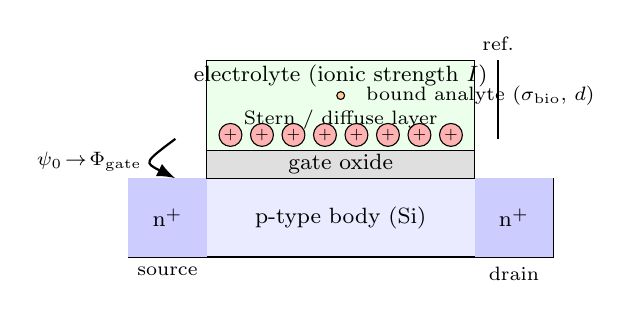
\begin{tikzpicture}[font=\footnotesize,>=Latex,node distance=0pt]
% semiconductor
\fill[blue!8] (0,0) rectangle (5.4,1.0);
\draw (0,0) rectangle (5.4,1.0);
\node at (2.7,0.5) {p-type body (Si)};
\fill[blue!20] (0,0) rectangle (1.0,1.0);
\fill[blue!20] (4.4,0) rectangle (5.4,1.0);
\node at (0.5,0.5) {n$^+$};
\node at (4.9,0.5) {n$^+$};
\node[below] at (0.5,0) {\scriptsize source};
\node[below] at (4.9,0) {\scriptsize drain};
% oxide
\fill[gray!25] (1.0,1.0) rectangle (4.4,1.35);
\draw (1.0,1.0) rectangle (4.4,1.35);
\node at (2.7,1.18) {gate oxide};
% electrolyte
\fill[green!8] (1.0,1.35) rectangle (4.4,2.5);
\draw (1.0,1.35) rectangle (4.4,2.5);
\node at (2.7,2.3) {electrolyte (ionic strength $I$)};
% double layer sketch
\foreach \x in {1.3,1.7,2.1,2.5,2.9,3.3,3.7,4.1}{
  \node[circle,draw,fill=red!30,inner sep=0.6pt] at (\x,1.55) {\tiny +};}
\node at (2.7,1.75) {\scriptsize Stern / diffuse layer};
% analyte
\node[circle,draw,fill=orange!40,inner sep=1pt] (bio) at (2.7,2.05) {};
\node[right] at (2.9,2.05) {\scriptsize bound analyte ($\sigma_{\mathrm{bio}}$, $d$)};
% reference electrode
\draw[thick] (4.7,1.5)--(4.7,2.5); \node[above] at (4.7,2.5){\scriptsize ref.};
% coupling arrow
\draw[->,thick] (0.6,1.5) .. controls (0.2,1.2) .. (0.6,1.0)
  node[left,midway]{\scriptsize $\psi_0\!\to\!\Phi_{\mathrm{gate}}$};
\end{tikzpicture}
\caption{Modelled ISFET/BioFET stack. The device core solves the semiconductor
and oxide; the interface model solves the electrolyte double layer and the bound
analyte; they couple at the oxide surface through the interfacial potential
$\psi_0$, mapped to the gate by Eq.~\eqref{eq:gate}.}
\label{fig:stack}
\end{figure}

\subsection{Governing equations}
The solver treats the steady-state semiconductor transport problem in the
quasi-Fermi-potential formulation. The primary nodal unknowns are the normalised
electrostatic potential $u=\psi/V_T$ and the electron and hole quasi-Fermi
potentials $v=\phi_n/V_T$, $w=\phi_p/V_T$, where $V_T=k_BT/q$ is the thermal
voltage. Carrier densities follow from Boltzmann statistics,
\begin{equation}
  n = n_i\,e^{\,u-v}, \qquad p = n_i\,e^{\,w-u},
  \label{eq:boltz}
\end{equation}
so that $np=n_i^2$ at equilibrium ($v=w=0$). With net doping
$C=(N_D-N_A)/n_i$, the coupled system is Poisson's equation and the two
continuity equations,
\begin{align}
  \nabla\!\cdot(\varepsilon\nabla\psi) &= -q\,(p-n+N_D-N_A), \label{eq:poisson}\\
  \nabla\!\cdot\mathbf{J}_n = +qR,\quad & \mathbf{J}_n = q\mu_n n\,\nabla\phi_n, \label{eq:jn}\\
  \nabla\!\cdot\mathbf{J}_p = -qR,\quad & \mathbf{J}_p = q\mu_p p\,\nabla\phi_p, \label{eq:jp}
\end{align}
with $R$ the net recombination rate (Shockley--Read--Hall and Auger; zero in the
ideal-diffusion limit). All quantities use the De Mari intrinsic
scaling~\cite{demari1968} so every unknown is $\mathcal{O}(1)$.

\subsection{Finite-element discretisation and coupled Newton solve}
The weak forms of \eqref{eq:poisson}--\eqref{eq:jp} are discretised with linear
triangular ($P_1$) elements and three-point Gauss quadrature, giving a global
$3N\times 3N$ residual $\mathbf{F}(u,v,w)=\mathbf{0}$. Because the carrier
densities \eqref{eq:boltz} are exponential in the unknowns, the exact analytic
Jacobian has a compact block structure whose entries are integrals of the shape
functions weighted by $e^{u-v}$ and $e^{w-u}$; DDM.SPC assembles this Jacobian
analytically and solves the fully coupled system by damped Newton iteration with
a per-step increment cap that prevents the exponential terms from overflowing on
a cold start. A robust thermal-equilibrium nonlinear-Poisson solve provides the
initial guess, and each bias point warm-starts from the previous solution. The
terminal current at a contact is extracted as the sum of the natural continuity
residuals over the contact nodes, which is conservative by construction.

\subsection{Insulated gate and the work-function transduction principle}
An insulated (MOS) gate imposes a Dirichlet condition on the electrostatic
potential only; the oxide carries no free carriers, and the quasi-Fermi unknowns
of oxide-only nodes are pinned. The gate node potential is referenced to the
metal work function $\Phi_m$,
\begin{equation}
  u_{\mathrm{gate}}=\frac{V_{\mathrm{gate}}}{V_T}
    +\frac{\Phi_{\mathrm{ref}}-\Phi_m}{V_T},\quad
  \Phi_{\mathrm{ref}}=\chi+\tfrac{1}{2}E_g+\tfrac{1}{2}V_T\ln\frac{N_c}{N_v}.
  \label{eq:gate}
\end{equation}
Equation~\eqref{eq:gate} is the hinge of every biosensor model here: a change
$\Delta\Phi$ in the effective gate work function shifts the threshold voltage by
$\Delta V_{\mathrm{th}}=\Delta\Phi/q$ to first order. In an ISFET the electrolyte
supplies that shift through the interfacial surface potential $\psi_0$
(Section~\ref{sec:gdl}), so we identify $\Delta\Phi_{\mathrm{gate}}=-q\,\psi_0$.

\subsection{Materials, contacts, and carrier statistics}
Each mesh region carries its own material (permittivity, affinity, band gap,
effective densities of states, mobilities, effective masses, and
recombination parameters), so heterojunctions are handled by a position-dependent
permittivity on the Poisson operator, per-element mobilities, and band-edge
offsets entering the density exponents via Anderson's electron-affinity rule.
Insulator regions (no free carriers) support MOS structures, and the boundary
library provides ohmic, insulated-gate, and rectifying Schottky contacts. For
degenerate layers---heavily-doped source/drain, strong inversion, or a
two-dimensional electron gas---Fermi--Dirac statistics can be selected, entering
as a degeneracy shift of the density exponent refreshed by the same outer
self-consistency loop as the quantum correction, and reducing to Boltzmann in the
non-degenerate limit. These capabilities are what let the same core serve the
homojunction diode used for validation (Section~\ref{sec:valid}) and the
MOS-gated ISFET used for the biosensor studies.

\subsection{Numerical methods and complexity}
\label{sec:numerics}
The coupled solve is summarised in Algorithm~\ref{alg:newton}. Two features make
it robust. First, the equilibrium initial guess is obtained from a nonlinear
Poisson solve with $v=w=0$, so $n=e^{u}$, $p=e^{-u}$; this places the potential
in the basin of attraction of the biased problem before the continuity equations
are switched on. Second, each Newton update is damped by a cap $\delta_{\max}$ on
the largest increment, which prevents the exponential density terms from
overflowing on a cold start while preserving the asymptotic quadratic
convergence once the iterate is close to the solution. The linear system at each
iteration is sparse ($\mathcal{O}(N)$ non-zeros for a quasi-uniform 2-D mesh of
$N$ nodes) and is solved by a sparse direct factorisation; the dominant cost per
bias point is therefore that of a handful of sparse solves. Bias sweeps
warm-start from the previous converged point, so the number of Newton iterations
per step is typically small (2--5) once past threshold. The exponential
dependence of the density on the unknowns means the discrete current is naturally
of Scharfetter--Gummel character~\cite{scharfetter1969}; here it arises from the
quasi-Fermi formulation rather than from an edge-based stabilisation.

\begin{algorithm}[t]
\caption{Coupled drift-diffusion solve at one bias point}
\label{alg:newton}
\begin{algorithmic}[1]
\State \textbf{Input:} mesh, doping $C$, contact biases, tolerance $\tau$
\State Solve nonlinear Poisson ($v=w=0$) $\to$ initial $u$; set $v=w=0$
\Repeat
  \State Assemble residual $\mathbf{F}(u,v,w)$ and analytic Jacobian $\mathbf{J}$
  \State Apply Dirichlet/contact conditions to $\mathbf{F},\mathbf{J}$
  \State Solve $\mathbf{J}\,\Delta\mathbf{x}=-\mathbf{F}$ (sparse direct)
  \State $\lambda \gets \min\!\big(1,\ \delta_{\max}/\|\Delta\mathbf{x}\|_\infty\big)$
         \Comment{damping}
  \State $(u,v,w) \gets (u,v,w) + \lambda\,\Delta\mathbf{x}$
\Until{$\|\Delta\mathbf{x}\|_\infty < \tau$}
\State \textbf{return} $(u,v,w)$; terminal current from contact residuals
\end{algorithmic}
\end{algorithm}

\subsection{Schr\"odinger--Poisson correction}
For thin, strongly-confined bodies the solver optionally adds a self-consistent
quantum-confinement correction. On slices cut across the confinement direction the
single-band effective-mass Schr\"odinger equation
\begin{equation}
  \Big[-\frac{\hbar^2}{2m^*}\frac{d^2}{dy^2}+U(y)\Big]\psi_i=E_i\psi_i
  \label{eq:schrod}
\end{equation}
is solved by linear FEM; the thermally-weighted subband density is renormalised to
preserve the local charge and enters the drift-diffusion assembly as an additive
quantum potential $\Lambda=\ln(n_{\mathrm{QM}}/n_{\mathrm{cl}})$ in the density
exponent. An outer Gummel-type loop recomputes $\Lambda$ from the updated
potential until convergence, following standard inversion-layer
practice~\cite{stern1972,ando1982,trellakis1997,ancona1987}; with $\Lambda=0$ the
classical solver is recovered exactly. This capability underpins the future
nanowire-BioFET study discussed in Section~\ref{sec:future}.

% =========================================================================
\section{Electrolyte Interface Model}
\label{sec:gdl}

The bare device solver treats the gate potential as an ideal control and
therefore predicts a unity analyte-to-threshold coupling. Real biosensors are
governed by the electrolyte interface, which we model with two coupled,
well-established ingredients.

\subsection{Site-binding surface charge}
A functionalised oxide presents amphoteric hydroxyl sites that protonate or
deprotonate according to the local proton activity~\cite{yates1974,fung1986}. For
total site density $N_s$, acid/base dissociation constants $K_a,K_b$, and surface
proton activity $h_s=h_{\mathrm{bulk}}\,e^{-q\psi_0/k_BT}$, the net surface charge
is
\begin{equation}
  \sigma_0(\psi_0)=qN_s\,
  \frac{h_s/K_a-K_b/h_s}{1+h_s/K_a+K_b/h_s},
  \label{eq:site}
\end{equation}
with point of zero charge $\mathrm{pH_{pzc}}=\tfrac12(\mathrm{p}K_a+\mathrm{p}K_b)$.
The surface buffer capacity $\beta_{\mathrm{int}}=-\,d\sigma_0/d\mathrm{pH}_s$
(large for high $N_s$ and small p$K$ spread) controls how Nernstian the sensor is.

\subsection{Gouy--Chapman--Stern double layer}
The surface charge is balanced by the diffuse layer through a Stern capacitance
$C_{\mathrm{St}}$ in series with the Gouy--Chapman diffuse charge~\cite{grahame1947,bard2001},
\begin{equation}
  \sigma_d(\psi_d)=-\sqrt{8\varepsilon_w\varepsilon_0 k_BT\,n_0}\,
  \sinh\!\Big(\frac{q\psi_d}{2k_BT}\Big),\quad
  \psi_0-\psi_d=\frac{\sigma_0}{C_{\mathrm{St}}}.
  \label{eq:gc}
\end{equation}
Charge neutrality $\sigma_0=-\sigma_d$ closes the system; the module solves the
scalar root
$\sigma_0(\psi_0)+\sigma_d(\psi_0-\sigma_0/C_{\mathrm{St}})=0$
self-consistently for $\psi_0$ at each pH using Brent's method (the site charge is
bounded, so $\psi_0$ remains physical).

\subsection{Sub-Nernstian response and the Debye limit}
The Nernst limit is $2.303\,k_BT/q\approx\SI{59.5}{mV/pH}$ at \SI{298}{K}; the
actual response is reduced by the van Hal sensitivity parameter
$\alpha\in(0,1]$~\cite{vanhal1996},
\begin{equation}
  \frac{d\psi_0}{d\mathrm{pH}}=-2.303\,\frac{k_BT}{q}\,\alpha,\quad
  \alpha=\Big(1+\frac{2.303\,k_BT\,C_{\mathrm{dl}}}{q^2\beta_{\mathrm{int}}}\Big)^{-1}.
  \label{eq:alpha}
\end{equation}
Equation~\eqref{eq:alpha} follows from a small-signal charge balance at the
surface: a change in surface pH perturbs the site charge through the buffer
capacity $\beta_{\mathrm{int}}$, which must be balanced by the double-layer charge
through the differential capacitance $C_{\mathrm{dl}}$. The two capacitances form
a divider, and the fraction of the ideal Nernstian potential that appears at the
surface is $\alpha=\beta_{\mathrm{int}}/(\beta_{\mathrm{int}}+q^2 C_{\mathrm{dl}}/(2.303\,k_BT))$,
which rearranges to Eq.~\eqref{eq:alpha}. A surface with abundant, weakly-spread
sites (large $\beta_{\mathrm{int}}$) approaches the Nernst limit; a poorly-buffered
surface such as SiO$_2$ does not. This is the compact explanation for the oxide
ordering measured in Table~\ref{tab:gdl}.

A biomolecule of charge-sheet density $\sigma_{\mathrm{bio}}$ captured a distance
$d$ from the surface contributes, in the linearised Debye--H\"uckel limit,
\begin{equation}
  \Delta\psi_{\mathrm{bio}}=\frac{\sigma_{\mathrm{bio}}}{\varepsilon_w\varepsilon_0\kappa}\,
  e^{-\kappa d},\quad
  \lambda_D=\kappa^{-1}=\sqrt{\frac{\varepsilon_w\varepsilon_0 k_BT}{2q^2N_AI}},
  \label{eq:debye}
\end{equation}
with $\lambda_D\approx 0.30/\sqrt{I[\mathrm{M}]}$~nm at room temperature. When the
ionic strength $I$ rises so that $\lambda_D<d$, the response collapses --- the
Debye-screening limit of Section~\ref{sec:related}.

\subsection{Coupling to the device solver}
The self-consistent surface potential $\psi_0$ enters the device gate as the
effective work-function shift $\Delta\Phi_{\mathrm{gate}}=-q\psi_0$
(Eq.~\eqref{eq:gate}), and the coupled model then produces a drain-current
transfer curve whose threshold is set by the electrolyte. This one-way coupling
(interface potential $\to$ gate) is appropriate in the sub-threshold and
low-current regime relevant to sensing, where the channel draws negligible
interfacial current and the double layer is in quasi-equilibrium. The full
device--electrolyte evaluation is summarised in Algorithm~\ref{alg:coupled}: for
each analyte state the electrolyte root \eqref{eq:gc} is solved once, its
potential is mapped to a gate work function, and the device transfer curve is
computed by Algorithm~\ref{alg:newton}; the threshold and its analyte
sensitivity are then extracted from the curve.

\begin{algorithm}[t]
\caption{Coupled device--electrolyte biosensor evaluation}
\label{alg:coupled}
\begin{algorithmic}[1]
\State \textbf{Input:} oxide $(N_s,\mathrm{p}K_a,\mathrm{p}K_b,C_{\mathrm{St}})$,
       analyte set $\{$pH$,I,\sigma_{\mathrm{bio}},d\}$, gate reference $\Phi_0$
\ForAll{analyte states}
  \State Solve $\sigma_0(\psi_0)+\sigma_d(\psi_0-\sigma_0/C_{\mathrm{St}})=0$
         for $\psi_0$ \Comment{Brent}
  \State Add Debye term $\Delta\psi_{\mathrm{bio}}=(\sigma_{\mathrm{bio}}/\varepsilon_w\varepsilon_0\kappa)e^{-\kappa d}$
  \State $\Phi_{\mathrm{gate}} \gets \Phi_0 - q(\psi_0+\Delta\psi_{\mathrm{bio}})$
  \State Compute $I_D(V_G)$ by Algorithm~\ref{alg:newton} with $\Phi_{\mathrm{gate}}$
  \State Extract $V_{\mathrm{th}}$ (constant-current), $S$, $I_{\mathrm{on}}$
\EndFor
\State \textbf{return} $V_{\mathrm{th}}$ vs.\ analyte; sensitivity $dV_{\mathrm{th}}/d(\text{analyte})$
\end{algorithmic}
\end{algorithm}

% =========================================================================
\section{Software Architecture}
\label{sec:arch}

The framework is organised as a small Python package (device core, materials,
mesh I/O, FEM primitives, physics assembly, recombination, quantum correction,
boundary conditions, solver, and post-processing) plus a set of application
scripts. The electrolyte model is a self-contained module that depends only on
\textsc{NumPy}/\textsc{SciPy}~\cite{harris2020,virtanen2020}; the device core adds
\textsc{Gmsh}~\cite{geuzaine2009} for unstructured meshes but also ships a
built-in structured mesh generator so that simple studies run with no external
mesher. Four application programs form a fidelity ladder from an idealised
demonstration to a physically realistic biosensor; they are compared in
Table~\ref{tab:programs}. This separation---an idealised front-end for intuition,
a full device for figures of merit, an electrolyte module for the sensing
chemistry, and a coupled driver for the realistic device---keeps each concern
independently testable and is what makes the workflow suitable for teaching as
well as design.

\begin{table}[t]
\centering
\caption{The four application programs and their roles.}
\label{tab:programs}
\footnotesize
\renewcommand{\arraystretch}{1.25}
\begin{tabular}{@{}p{1.9cm}p{2.0cm}p{3.0cm}@{}}
\toprule
Program & Role & Key physics / output \\
\midrule
MOS-cap front-end & transduction demo & Poisson+gate; $\psi_s$, $\Delta V_{\mathrm{th}}$ \\
Transfer-curve model & full device & +continuity; $I_D(V_G)$, $S$, sensitivity \\
Double-layer module & electrolyte interface & site-binding + GCS; $\psi_0$, $\alpha$, $\lambda_D$ \\
Coupled driver & realistic biosensor & device $\times$ electrolyte; sub-Nernstian $dV_{\mathrm{th}}/d\mathrm{pH}$ \\
\bottomrule
\end{tabular}
\end{table}

% =========================================================================
\section{Solver Validation}
\label{sec:valid}

Because the device solver is a research code rather than an established package,
we first establish quantitative agreement with analytic semiconductor physics on
a two-dimensional silicon p-n diode. Four canonical checks are used
(Fig.~\ref{fig:bench}, Table~\ref{tab:bench}):

\begin{enumerate}
  \item \textbf{Built-in potential.} The equilibrium potential drop matches the
  analytic $V_{bi}=V_T\ln(N_AN_D/n_i^2)$ to within \SI{6}{mV} across
  $N_A=N_D=10^{15}$--$10^{17}\,\mathrm{cm^{-3}}$.
  \item \textbf{Law of mass action.} At equilibrium
  $\max|np/n_i^2-1|=3.3\ee{-16}$, i.e.\ machine precision.
  \item \textbf{Ideality factor.} The forward-bias current is exponential with
  ideality $n=1.005$ (ideal-diffusion value $1.000$).
  \item \textbf{Current conservation.} The two terminal currents are equal and
  opposite to $\max|I_a+I_c|/|I_a|=5\ee{-5}$.
\end{enumerate}

\begin{table}[t]
\centering
\caption{Validation of the device solver against analytic physics
(2-D Si p-n diode).}
\label{tab:bench}
\footnotesize
\begin{tabular}{@{}p{3.2cm}p{2.6cm}p{1.7cm}@{}}
\toprule
Check & Analytic reference & Result \\
\midrule
Built-in potential & $V_T\ln(N_AN_D/n_i^2)$ & $\le\SI{6}{mV}$ err \\
Mass action & $np=n_i^2$ & $3.3\ee{-16}$ \\
Ideality factor & $n=1$ (ideal) & $1.005$ \\
Current conservation & $I_a=-I_c$ & $5\ee{-5}$ \\
\bottomrule
\end{tabular}
\end{table}

\begin{figure}[t]
\centering
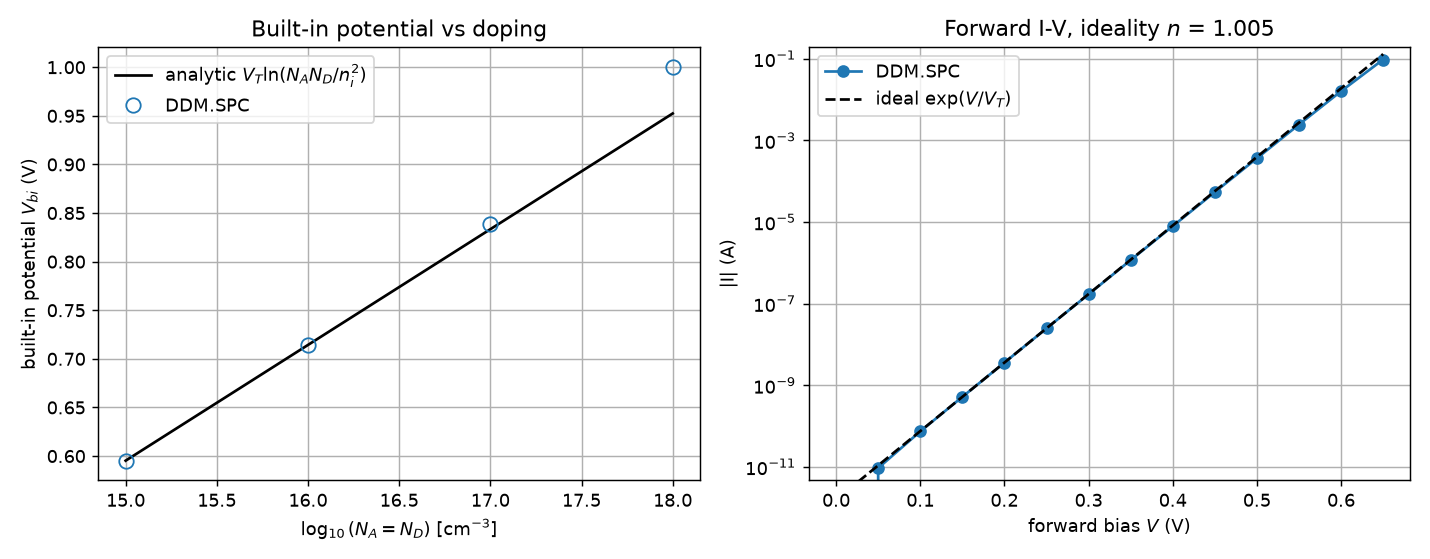
\includegraphics[width=\columnwidth]{figures/benchmark_ddmspc.png}
\caption{Validation of the device solver. Left: built-in potential versus doping;
the solver (circles) lies on the analytic curve through $10^{17}\,\mathrm{cm^{-3}}$.
Right: forward-bias $I$--$V$ on the ideal $\exp(V/V_T)$ law, giving ideality
$n=1.005$.}
\label{fig:bench}
\end{figure}

On a single workstation core the equilibrium solve for the diode completes in a
few seconds, a full three-curve ISFET transfer sweep in under three minutes, and
the entire electrolyte analysis in well under a second; the coupled
device--electrolyte chain over several pH points runs in a few minutes. These
times, modest because the problems are two-dimensional and the meshes are small,
are what make the framework practical for interactive design exploration and for
classroom use rather than only for batch runs.

The one visible departure, at $N_A=N_D=10^{18}\,\mathrm{cm^{-3}}$, where the
numeric $V_{bi}$ exceeds the analytic value by $\sim\!\SI{48}{mV}$, is expected
and instructive: the closed-form $V_T\ln(N_AN_D/n_i^2)$ is the non-degenerate
(Boltzmann) approximation, and at $10^{18}\,\mathrm{cm^{-3}}$ the Fermi level
approaches the band edge, where that formula itself breaks down and Fermi--Dirac
statistics are required. The benchmark thus confirms correct behaviour in the
regime where the analytic law is exact and exhibits the expected onset of its
breakdown at degeneracy. Together these checks provide the credibility baseline
needed before trusting the device curves that follow.

% =========================================================================
\section{Results}
\label{sec:results}

We now apply the framework to the ISFET/BioFET, progressing from an idealised
front-end to the electrolyte-limited full device. The device and interface
parameters used throughout are listed in Table~\ref{tab:params}; the oxide
$(N_s,\mathrm{p}K_a,\mathrm{p}K_b)$ triples are representative literature-consistent
values chosen to reproduce the known sensitivity ordering, not fits to a specific
fabrication.

\begin{table}[t]
\centering
\caption{Simulation parameters.}
\label{tab:params}
\footnotesize
\begin{tabular}{@{}lll@{}}
\toprule
Group & Parameter & Value \\
\midrule
Device & body doping $N_A$ & $10^{17}\,\mathrm{cm^{-3}}$ \\
       & source/drain $N_D$ & $10^{20}\,\mathrm{cm^{-3}}$ \\
       & drain bias $V_D$ & \SI{0.1}{V} \\
       & width $W$ & \SI{1}{\micro m} \\
Electrolyte & temperature $T$ & \SI{298}{K} \\
       & $\varepsilon_w$ & 78.5 \\
       & Stern cap.\ $C_{\mathrm{St}}$ & \SIrange{0.2}{0.4}{F/m^2} \\
Oxides & Ta$_2$O$_5$ $(N_s,\mathrm{p}K_a,\mathrm{p}K_b)$ & $(10^{19},2,4)$ \\
       & SiO$_2$ $(N_s,\mathrm{p}K_a,\mathrm{p}K_b)$ & $(2\ee{17},-1,7)$ \\
Analyte & bound charge $\sigma_{\mathrm{bio}}$ & $-0.01\,\mathrm{C/m^2}$ \\
       & distance $d$ & \SI{3}{nm} (nominal) \\
\bottomrule
\end{tabular}
\end{table}

\subsection{MOS-capacitor front-end}
The transduction principle is isolated in a MOS-capacitor structure (p-Si body
under a gate oxide) solved on a structured mesh. Modelling analyte binding as a
gate work-function step of \SI{+0.20}{eV}, the silicon surface potential versus
gate voltage shifts rigidly by the same amount (Fig.~\ref{fig:moscap}): the
extracted threshold shift is \SI{+200}{mV}, i.e.\ near-unity coupling, confirming
Eqs.~\eqref{eq:gate}--\eqref{eq:site}. The characteristic sweeps the silicon
surface through accumulation, depletion, and inversion as the gate bias rises,
and the analyte step translates the whole curve laterally without changing its
shape---the signature of a pure work-function shift and the reason the extracted
sensitivity is independent of the chosen readout point in this idealised limit.

\begin{figure}[t]
\centering
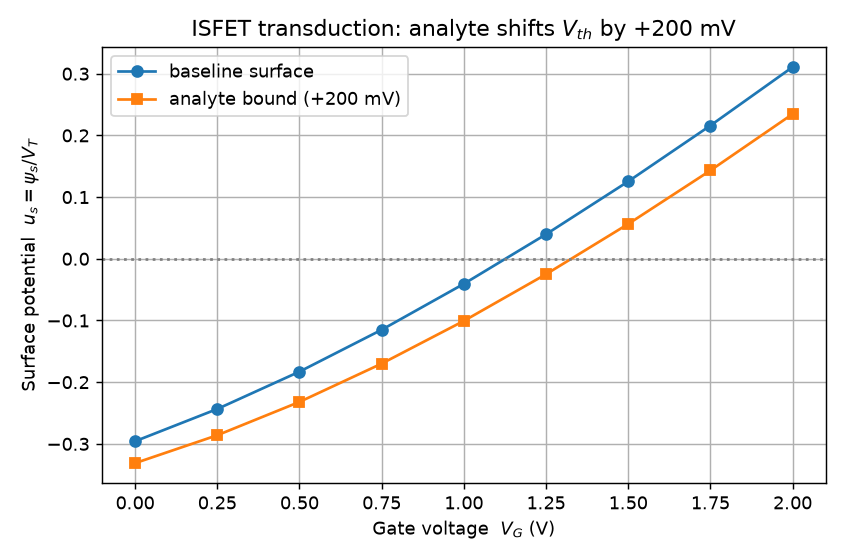
\includegraphics[width=0.86\columnwidth]{figures/isfet_moscap.png}
\caption{MOS-capacitor front-end: an analyte-induced gate work-function step
rigidly translates the surface-potential characteristic, isolating the ISFET
transduction principle.}
\label{fig:moscap}
\end{figure}

\subsection{Full-device transfer characteristics}
The complete ISFET (n$^+$ source/drain, p body, gate oxide) is solved on a tuned
short-channel mesh. Figure~\ref{fig:transfer} shows the drain-current transfer
curves $I_D(V_G)$ for a series of analyte-induced work-function steps, in linear
and semilogarithmic form. Table~\ref{tab:transfer} lists the extracted figures of
merit. The analyte-to-threshold coupling is exactly unity
($dV_{\mathrm{th}}/d\Phi=1.000$) --- the ideal limit, because the bare device has
no electrolyte --- and the sub-threshold swing $S\approx\SI{135}{mV/dec}$ exceeds
the \SI{60}{mV/dec} thermal limit, reflecting the short-channel geometry. The
semilogarithmic plot (Fig.~\ref{fig:transfer}, right) makes the mechanism
explicit: below threshold the three curves are parallel and rigidly displaced
along the gate axis by the work-function step, while above threshold they
converge as the channel enters strong conduction. The elevated swing is a genuine
device-physics result of the sub-\SI{200}{nm} channel and the associated
drain-induced barrier lowering; a long-channel device would approach the thermal
limit, and adding such a geometry is a natural way to strengthen the device-side
validation. Because the sensor signal is the sub-threshold \emph{shift} rather
than the absolute swing, the transduction remains faithful even when $S$ is
degraded, though the resolution analysis of Section~\ref{sec:resolution} shows a
smaller $S$ would improve the detection limit.

\begin{figure*}[t]
\centering
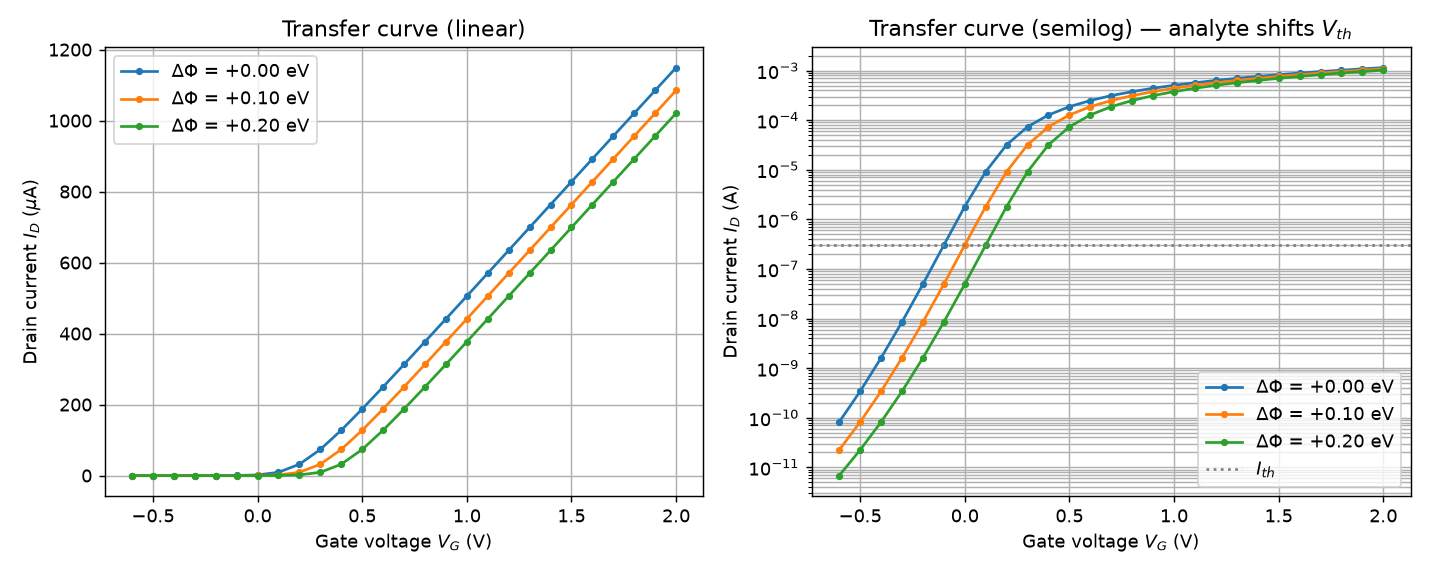
\includegraphics[width=0.92\textwidth]{figures/isfet_transfer.png}
\caption{Full-device ISFET transfer curves $I_D(V_G)$ (linear, left; semilog,
right) for analyte-induced work-function steps $\Delta\Phi=0,0.1,0.2$~eV at
$V_D=\SI{0.1}{V}$, $W=\SI{1}{\micro m}$. The threshold shift is the sensor signal;
the coupling is unity because the bare device lacks the electrolyte.}
\label{fig:transfer}
\end{figure*}

\begin{table}[t]
\centering
\caption{Transfer-curve figures of merit ($W=\SI{1}{\micro m}$, $V_D=\SI{0.1}{V}$).}
\label{tab:transfer}
\footnotesize
\begin{tabular}{@{}rrrrr@{}}
\toprule
$\Delta\Phi$ (eV) & $V_{\mathrm{th}}$ (V) & $\Delta V_{\mathrm{th}}$ (mV) & $S$ (mV/dec) & $I_{\mathrm{on}}$ (A) \\
\midrule
$+0.00$ & $-0.099$ & 0   & 135 & $1.15\ee{-3}$ \\
$+0.10$ & $+0.001$ & 100 & 135 & $1.09\ee{-3}$ \\
$+0.20$ & $+0.101$ & 200 & 135 & $1.02\ee{-3}$ \\
\midrule
\multicolumn{5}{@{}l}{Sensitivity $dV_{\mathrm{th}}/d\Phi=1.000$~V/V (ideal, unity coupling).}\\
\bottomrule
\end{tabular}
\end{table}

\subsection{Electrolyte-limited biosensor}
Adding the electrolyte model makes the coupling realistically sub-unity.
Figure~\ref{fig:gdl} (left) shows the site-binding surface potential
$\psi_0(\mathrm{pH})$ for four representative gate oxides; its slope is the
sub-Nernstian sensitivity, summarised in Table~\ref{tab:gdl}. The ordering
Ta$_2$O$_5>$ Al$_2$O$_3>$ Si$_3$N$_4>$ SiO$_2$ and the magnitudes
(\SIrange{31}{57}{mV/pH}) reproduce the well-known experimental
trend~\cite{bousse1983,vanhal1996}. Figure~\ref{fig:gdl} (right) and
Table~\ref{tab:debye} show the Debye-screening collapse: a fixed bound charge at
$d=\SI{3}{nm}$ produces \SI{-101}{mV} at \SI{1}{mM} but only \SI{-0.25}{mV} at
physiological ionic strength ($\lambda_D\approx\SI{0.8}{nm}$), a
$\sim\!400\times$ reduction, consistent with the nanowire-FET
observations of Stern~\emph{et al.}~\cite{stern2007debye}. When the electrolyte
model drives the full device solve, the transistor threshold sensitivity is
electrolyte-limited (Table~\ref{tab:chain}): \SI{57.4}{mV/pH} for Ta$_2$O$_5$ and
\SI{24.6}{mV/pH} for SiO$_2$, both below the Nernst limit, unlike the
ideal-coupling device of Table~\ref{tab:transfer}. The near-linear
$\psi_0(\mathrm{pH})$ characteristics of Fig.~\ref{fig:gdl} (left) confirm that a
single sensitivity slope is a good descriptor over the physiological pH range,
and their spread---steep and near-Nernstian for Ta$_2$O$_5$, shallow for
SiO$_2$---directly reflects the buffer-capacity ordering through $\alpha$.

\begin{table}[t]
\centering
\caption{Full device--electrolyte chain: electrolyte-limited threshold
sensitivity (constant-current $V_{\mathrm{th}}$, pH 4/7/10).}
\label{tab:chain}
\footnotesize
\begin{tabular}{@{}lcc@{}}
\toprule
Gate oxide & Surface $d\psi_0/d\mathrm{pH}$ & Device $dV_{\mathrm{th}}/d\mathrm{pH}$ \\
\midrule
Ta$_2$O$_5$ & \SI{57.4}{mV/pH} & \SI{57.4}{mV/pH} \\
SiO$_2$     & \SI{31.6}{mV/pH} & \SI{24.6}{mV/pH} \\
\bottomrule
\end{tabular}
\end{table}

The small SiO$_2$ offset between the surface slope and the extracted device slope
arises from the constant-current threshold definition applied over a wide,
three-point pH range together with short-channel non-ideality, and bounds the
consistency of the one-way coupling in this regime.

\begin{figure*}[t]
\centering
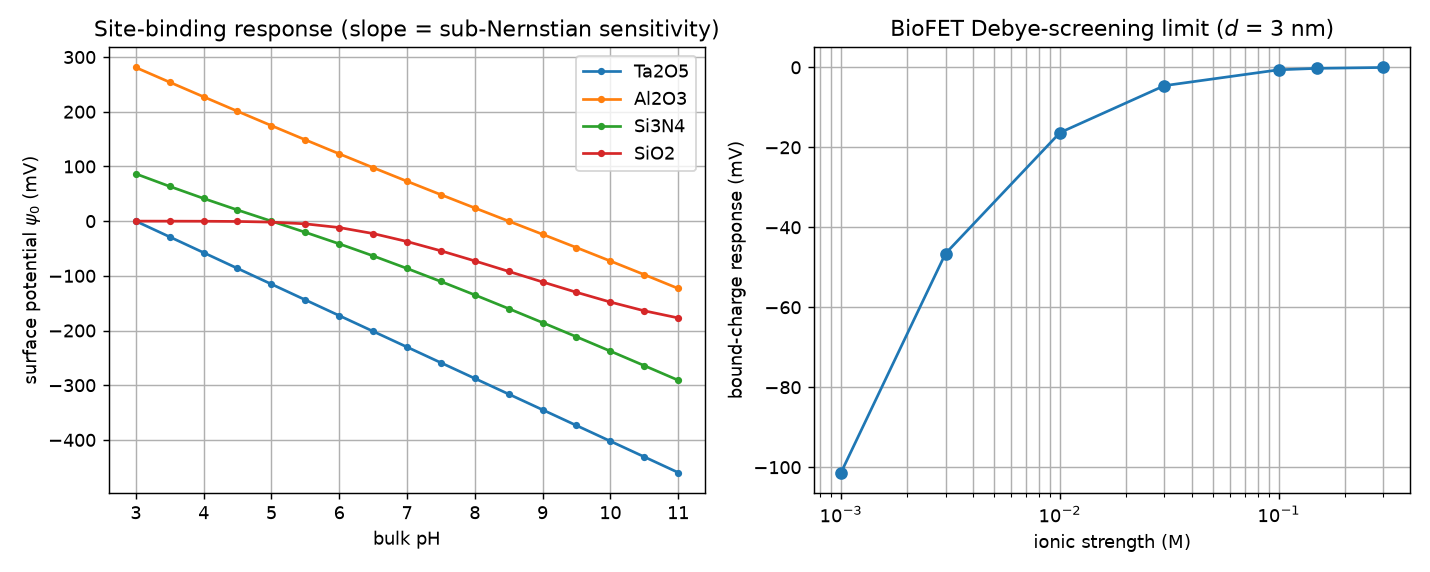
\includegraphics[width=0.92\textwidth]{figures/isfet_gdl.png}
\caption{Electrolyte double-layer model. Left: site-binding surface potential
$\psi_0(\mathrm{pH})$; the slope is the sub-Nernstian sensitivity. Right: the
Debye-screening limit --- a bound charge at $d=\SI{3}{nm}$ becomes undetectable as
increasing ionic strength shrinks $\lambda_D$ below $d$.}
\label{fig:gdl}
\end{figure*}

\begin{table}[t]
\centering
\caption{Sub-Nernstian pH sensitivity at pH~7, $I=\SI{0.15}{M}$
(Nernst limit \SI{59.2}{mV/pH}).}
\label{tab:gdl}
\footnotesize
\begin{tabular}{@{}lrr@{}}
\toprule
Gate oxide & Sensitivity (mV/pH) & $\alpha$ \\
\midrule
Ta$_2$O$_5$ & 57.4 & 0.97 \\
Al$_2$O$_3$ & 49.5 & 0.84 \\
Si$_3$N$_4$ & 46.9 & 0.79 \\
SiO$_2$     & 31.6 & 0.53 \\
\bottomrule
\end{tabular}
\end{table}

\begin{table}[t]
\centering
\caption{BioFET Debye screening: bound charge $-0.01\,\mathrm{C/m^2}$ at
$d=\SI{3}{nm}$.}
\label{tab:debye}
\footnotesize
\begin{tabular}{@{}rrr@{}}
\toprule
$I$ (M) & $\lambda_D$ (nm) & Response (mV) \\
\midrule
0.001 & 9.62 & $-101.3$ \\
0.010 & 3.04 & $-16.3$ \\
0.100 & 0.96 & $-0.61$ \\
0.150 & 0.79 & $-0.25$ \\
\bottomrule
\end{tabular}
\end{table}

\subsection{Coupling factor and resolution}
\label{sec:resolution}
The two device models bracket the sensitivity. The bare device
(Table~\ref{tab:transfer}) has coupling $g\equiv dV_{\mathrm{th}}/d\Phi=1$, so its
pH sensitivity would equal the full Nernst slope; the electrolyte-limited device
reduces this to $g\,\cdot 2.303(k_BT/q)\alpha$ with $\alpha<1$
(Eq.~\eqref{eq:alpha}), giving the measured \SIrange{24.6}{57.4}{mV/pH}. The
smallest resolvable analyte change follows from the transfer characteristic: a
current noise floor $\Delta I/I$ maps to a threshold resolution
$\Delta V_{\mathrm{th}}\approx S\log_{10}(1+\Delta I/I)$ through the sub-threshold
swing $S$, and thence to a surface-potential resolution
$\Delta\psi_0=\Delta V_{\mathrm{th}}/g$. With the simulated $S\approx\SI{135}{mV/dec}$
and a conservative \SI{1}{\percent} current resolution, the device resolves
$\Delta V_{\mathrm{th}}\approx\SI{0.6}{mV}$, i.e.\ a pH resolution of
$\sim\!0.01$--$0.02$ for a near-Nernstian oxide. This chain---noise floor,
sub-threshold swing, coupling, sensitivity---is exactly what the framework makes
computable end-to-end, and it identifies $S$ (device geometry) and $\alpha$
(surface chemistry) as the two independent levers on the detection limit.

% =========================================================================
\section{Discussion}
\label{sec:discussion}

\subsection{Design implications for disease detection}
The results map directly onto label-free diagnostic devices. Because the analyte
alters $\psi_0$ and hence the threshold via Eq.~\eqref{eq:gate}, the framework
lets a designer trade off the sensing chemistry and the device electrostatics in
one place: (i)~for \emph{pH and metabolic} assays, oxide choice sets the
sensitivity through $\alpha$ (Table~\ref{tab:gdl}); (ii)~for \emph{DNA-FET} and
\emph{ImmunoFET} assays, the Debye limit (Table~\ref{tab:debye}) dictates that
low ionic strength or short receptor--target distances are required for the
target charge to be visible; (iii)~for \emph{enzymatic (glucose)} sensors, the
local pH change produced by the enzymatic reaction is read out as in the pH case.
The unity-coupling device model (Table~\ref{tab:transfer}) and the
electrolyte-limited model bracket the achievable sensitivity, and the difference
between them quantifies exactly how much signal the double layer removes.

\subsection{Worked example: an ImmunoFET in physiological buffer}
To illustrate the model as a design aid, consider a cardiac-troponin ImmunoFET
operated in physiological buffer ($I=\SI{0.15}{M}$). The Debye length is
$\lambda_D\approx\SI{0.79}{nm}$ (Table~\ref{tab:debye}). An antibody-captured
antigen sits well beyond this length: with a typical antibody footprint the
effective charge centroid is $d\approx$ \SIrange{5}{12}{nm} from the oxide, so the
screening factor $e^{-d/\lambda_D}$ is of order $10^{-3}$ or smaller, and the
model predicts a surface-potential signal below the \SI{0.6}{mV} resolution
estimated in Section~\ref{sec:resolution}---i.e.\ the assay is essentially
undetectable at physiological ionic strength. Reducing the buffer to
$I=\SI{1}{mM}$ raises $\lambda_D$ to \SI{9.6}{nm}, bringing $d\lesssim\lambda_D$
and the predicted signal into the \SIrange{10}{100}{mV} range
(Table~\ref{tab:debye}). The model thus reproduces, quantitatively, the
well-documented requirement to sense in low-ionic-strength media or with
charge-proximity strategies~\cite{stern2007debye,gao2015}, and lets a designer
estimate the required buffer dilution before fabrication.

\subsection{A biosensor design map}
The interplay of binding distance and ionic strength can be condensed into a
single design chart. Figure~\ref{fig:designmap} plots the predicted
surface-potential response for a fixed bound charge as a function of the analyte
binding distance $d$, for four ionic strengths, against the \SI{0.6}{mV}
resolution floor estimated in Section~\ref{sec:resolution}. The region above the
floor is the detectable design space. At physiological ionic strength it is
confined to $d\lesssim\SI{2}{nm}$---smaller than a typical antibody---whereas at
\SI{1}{mM} the entire \SIrange{0.5}{12}{nm} range is detectable. Such a chart,
produced in under a second by the electrolyte module, turns the abstract Debye
constraint into an actionable specification on receptor size and buffer
condition.

\begin{figure}[t]
\centering
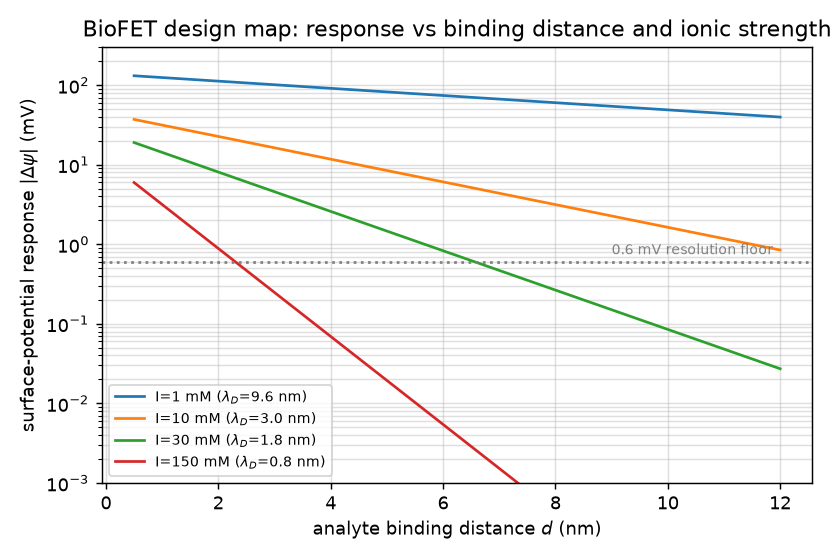
\includegraphics[width=0.98\columnwidth]{figures/designmap.png}
\caption{BioFET design map: predicted surface-potential response versus analyte
binding distance $d$ for four ionic strengths, against the \SI{0.6}{mV}
resolution floor (dotted). The detectable design space (above the floor)
collapses toward the surface as ionic strength rises.}
\label{fig:designmap}
\end{figure}

\subsection{Design guidelines}
Table~\ref{tab:guidelines} distils the results into practical guidance for four
common assay classes. The recurring message is that device and interface must be
co-designed: a high-$\alpha$ oxide maximises pH sensitivity but does nothing for
a charge-based assay that is Debye-limited, while a charge-based assay in
physiological buffer demands either a reduced ionic strength, a short
receptor--target distance, or a debye-length-extending strategy such as a porous
membrane~\cite{gao2015}. The framework makes these trade-offs quantitative in a
single tool.

\begin{table}[t]
\centering
\caption{Design guidance derived from the model for common assay classes.}
\label{tab:guidelines}
\footnotesize
\renewcommand{\arraystretch}{1.25}
\begin{tabular}{@{}p{1.6cm}p{2.0cm}p{3.2cm}@{}}
\toprule
Assay & Dominant limit & Design lever \\
\midrule
pH / metabolic & buffer capacity $\alpha$ & high-$N_s$ oxide (Ta$_2$O$_5$/Al$_2$O$_3$) \\
DNA-FET & Debye screening & low $I$; short probe; $d<\lambda_D$ \\
ImmunoFET & Debye + coverage & low $I$; small receptor; high capture density \\
Enzymatic (glucose) & local pH gain & high-$\alpha$ oxide + enzyme loading \\
\bottomrule
\end{tabular}
\end{table}

\subsection{Practical non-idealities}
Several effects important in real ISFET operation are outside the present
steady-state, mean-field scope but are worth situating relative to the model.
\emph{Temperature} enters through $V_T$, $n_i$, the mobilities, and the
electrolyte dissociation constants; the framework can be re-run at any temperature
by setting the material and interface parameters accordingly, but does not yet
model self-heating. \emph{Drift and hysteresis}---the slow, sub-Nernstian
wander of the ISFET response attributed to buried-site hydration and ion
migration in the insulator~\cite{jamasb1998}---are dynamic phenomena requiring a
transient solve and an extended interface model, and set a practical floor on the
resolution estimated in Section~\ref{sec:resolution}. The \emph{reference
electrode} is assumed ideal here, contributing a constant offset; in integrated
or reference-electrode-free designs its non-idealities must be added to the gate
term of Eq.~\eqref{eq:gate}. Compact ISFET models developed for circuit
simulation capture several of these effects
phenomenologically~\cite{martinoia2005,chin2001}, and could be combined with the
physical device model presented here. Finally, the enhanced sensitivity reported
for aggressively-scaled nanoscale FET biosensors has both electrostatic and
quantum origins~\cite{shoorideh2014,nair2007}; disentangling them is precisely
the role envisaged for the Schr\"odinger--Poisson capability of
Section~\ref{sec:device}.

\subsection{Relation to existing tools}
Compared with commercial TCAD~\cite{sentaurus,comsol}, the present framework is
far more limited in scope but is open, lightweight, and ships the electrolyte
coupling as a first-class component rather than as user scripting. Compared with
open device solvers~\cite{sanchez2016,charon2020}, it adds the integrated
site-binding/double-layer front-end and a worked biosensor workflow.
Table~\ref{tab:tools} positions it against representative tools. Its intended
role is complementary: a reproducible, license-free platform for biosensor
device--interface co-design and for teaching, and a transparent reference against
which larger tools can be cross-checked.

\begin{table}[t]
\centering
\caption{Positioning against representative device-simulation tools.}
\label{tab:tools}
\footnotesize
\renewcommand{\arraystretch}{1.25}
\begin{tabular}{@{}p{1.7cm}cccc@{}}
\toprule
Tool & Open & Light & Quantum & Electrolyte \\
\midrule
Sentaurus~\cite{sentaurus} & no & no & yes & scripted \\
COMSOL~\cite{comsol} & no & no & yes & scripted \\
DEVSIM~\cite{sanchez2016} & yes & yes & partial & scripted \\
Charon~\cite{charon2020} & yes & no & partial & scripted \\
This work & yes & yes & yes (S--P) & built-in \\
\bottomrule
\end{tabular}
\end{table}

% =========================================================================
\section{Limitations and Future Work}
\label{sec:future}

Several limitations bound the present scope and define the roadmap. The device
solver is steady-state, so binding kinetics, impedance/$C$--$V$, and
low-frequency noise are out of scope; a transient continuity solve is the natural
extension. There is no optical generation term, so photodetector-style biosensors
are not yet covered. The electrolyte model is mean-field: the two-p$K$
site-binding parameters $(N_s,\mathrm{p}K_a,\mathrm{p}K_b)$ are representative
values chosen to reproduce the known oxide ordering and sensitivity ranges rather
than fitted to a specific fabrication, and the coupling to the device is one-way.
The mean-field electrolyte treatment also neglects ion correlations, finite ion
size, and Stern-layer dispersion, which become significant at high ionic strength
and for multivalent ions; more elaborate modified-Poisson--Boltzmann descriptions
could be substituted for Eq.~\eqref{eq:gc} within the same coupling scheme.
Most importantly, the biosensor results are validated against the analytic
Nernst and Debye limits and the device solver against analytic diode physics, but
not yet against measured device data; experimental calibration---extracting
$(N_s,\mathrm{p}K_a,\mathrm{p}K_b,C_{\mathrm{St}})$ from a titration and the
device parameters from a fabricated transistor---is required before quantitative,
device-specific design claims can be made. Until then the framework is best
regarded as a physically-grounded design-space explorer and teaching tool rather
than a predictive replacement for calibrated TCAD. Finally, the
Schr\"odinger--Poisson capability of Section~\ref{sec:device} enables a
quantum-corrected nanowire-BioFET study --- quantifying how carrier confinement in
a few-nanometre body modifies sensitivity~\cite{nair2007,stern1972} --- which we
identify as the most promising direction for a novel, physics-driven result.

% =========================================================================
\section{Conclusion}
\label{sec:conclusion}

We have presented an open, validated, finite-element drift-diffusion and
Schr\"odinger--Poisson framework for ISFET/BioFET simulation, coupled to a
self-consistent site-binding and Gouy--Chapman--Stern electrolyte model. The
device solver reproduces analytic semiconductor physics quantitatively (built-in
potential to \SI{6}{mV}, mass action to $10^{-16}$, ideality $1.005$, current
conservation to $10^{-5}$), and the coupled model recovers the two defining
non-idealities of real biosensors --- sub-Nernstian pH response and the
Debye-screening detection limit --- from first principles. Because the framework
is compact, dependency-minimal, and openly released with all scripts and data, it
offers a reproducible platform for biosensor device--electrolyte co-design and for
teaching, and a foundation for the quantum-corrected nanowire-BioFET study
outlined above. More broadly, the work illustrates a modelling pattern that is
likely to recur as electronic biosensors proliferate: a validated but lightweight
device solver, coupled to a physically-based interface model, can turn qualitative
design intuition into quantitative, reproducible predictions without the overhead
of a full commercial TCAD flow. We hope the openness of the framework lowers the
barrier for other groups to extend it---toward transient operation, additional
surface chemistries, and, ultimately, experimental calibration.

% =========================================================================
\section*{Reproducibility and Code Availability}
All source code, meshes, material files, and the scripts that generate every
figure and table in this paper are openly available in the project repository,
along with build instructions. The four programs used here are the MOS-capacitor
front-end, the full-device transfer-curve model, the electrolyte double-layer
module, and the coupled device--electrolyte driver; the validation benchmark of
Section~\ref{sec:valid} is provided as a standalone script.

% =========================================================================
\appendices
\section{De Mari Scaling and the Analytic Jacobian}
\label{app:scaling}
The solver works in De Mari intrinsic units~\cite{demari1968}: potentials are
scaled by $V_T$, lengths by the intrinsic Debye length
$L_D=\sqrt{\varepsilon V_T/qn_i}$, and carrier densities by $n_i$, so that every
unknown is $\mathcal{O}(1)$ and the assembled system is well conditioned across
many doping decades. In these units the Poisson residual for node $i$ is
$\int(\nabla N_i\!\cdot\!\nabla u + N_i(n-p-C))\,d\Omega$ and the two continuity
residuals are $\int\mu\, n\,\nabla N_i\!\cdot\!\nabla v\,d\Omega$ and the hole
analogue.

Because $n=e^{u-v}$ and $p=e^{w-u}$, the element Jacobian has the block form
\begin{equation}
J=\begin{bmatrix} K_{uu} & K_{uv} & K_{uw}\\ K_{vu} & K_{vv} & 0\\ K_{wu} & 0 & K_{ww}\end{bmatrix},
\end{equation}
with, for example,
$(K_{uu})_{ik}=\int\nabla N_i\!\cdot\!\nabla N_k\,d\Omega+\int N_iN_k(e^{u-v}+e^{w-u})\,d\Omega$
and $(K_{uv})_{ik}=-\int N_iN_k e^{u-v}\,d\Omega$. All entries are evaluated
analytically at the three-point Gauss nodes, so the Newton iteration is exact and
retains quadratic convergence. Enabling generation--recombination makes the
previously-zero $K_{vw},K_{wv}$ blocks non-zero through the analytic derivatives
$\partial R/\partial n,\ \partial R/\partial p$; the quantum and Fermi--Dirac
corrections enter as frozen additive shifts in the density exponents and hence
leave the Jacobian structure unchanged within a Newton solve, being refreshed by
the outer self-consistency loop.

\section{Reproducing the Results}
\label{app:repro}
Each figure and table is produced by a single script: the validation benchmark
(Fig.~\ref{fig:bench}, Table~\ref{tab:bench}); the MOS-capacitor front-end
(Fig.~\ref{fig:moscap}); the transfer-curve model (Fig.~\ref{fig:transfer},
Table~\ref{tab:transfer}); and the electrolyte/coupled driver
(Figs.~\ref{fig:gdl}, \ref{fig:designmap}, Tables~\ref{tab:gdl}--\ref{tab:chain}).
The device scripts require the device package and \textsc{Gmsh}; the electrolyte
module requires only \textsc{NumPy}/\textsc{SciPy}. Run times are reported in
Section~\ref{sec:valid}.

\bibliographystyle{IEEEtran}
\bibliography{refs}

\end{document}
